\documentclass[aspectratio=169]{beamer}

% ── Fonts ──────────────────────────────────────────────────────────────────────
\usepackage[T1]{fontenc}
\usepackage{helvet}
\renewcommand{\familydefault}{\sfdefault}

% ── Packages ───────────────────────────────────────────────────────────────────
\usepackage{graphicx}
\usepackage{tikz}
\usepackage{xcolor}
\usepackage{booktabs}

% ── Color palette ──────────────────────────────────────────────────────────────
\definecolor{utblue}{HTML}{005F86}
\definecolor{utlightblue}{HTML}{00A9CE}
\definecolor{utred}{HTML}{BF5700}
\definecolor{utgray}{HTML}{9CADB7}
\definecolor{bgwhite}{HTML}{FFFFFF}
\definecolor{textdark}{HTML}{1A1A2E}

% ── Theme ──────────────────────────────────────────────────────────────────────
\usetheme{default}
\setbeamercolor{background canvas}{bg=bgwhite}
\setbeamercolor{normal text}{fg=textdark}
\setbeamercolor{frametitle}{fg=utblue}
\setbeamercolor{itemize item}{fg=utred}
\setbeamercolor{itemize subitem}{fg=utlightblue}
\setbeamerfont{frametitle}{size=\Large, series=\bfseries}
\setbeamertemplate{navigation symbols}{}
\setbeamertemplate{itemize item}{\small\textbullet}
\setbeamertemplate{itemize subitem}{\scriptsize\textbullet}

% ── Footer (aparece en todas las slides excepto portada e indice) ──────────────
\newcommand{\currentspeaker}{}
\newcommand{\setspeaker}[1]{\renewcommand{\currentspeaker}{#1}}

\newcommand{\showfooter}{%
  \setbeamertemplate{footline}{
    \begin{beamercolorbox}[wd=\paperwidth, ht=0.4pt]{normal text}
      \color{utlightblue}\rule{\paperwidth}{0.4pt}
    \end{beamercolorbox}
    \vspace{3pt}
    \hspace{8pt}
    {\scriptsize\color{utgray}
      \currentspeaker
      \quad\textbar\quad [MATERIA] \quad\textbar\quad UT Austin
    }
    \hfill
    {\scriptsize\color{utgray}\insertframenumber\hspace{8pt}}
    \vspace{4pt}
  }
}

\newcommand{\hidefooter}{%
  \setbeamertemplate{footline}{}
}

% ── Accent rule ────────────────────────────────────────────────────────────────
\newcommand{\accentrule}{%
  
\begin{tikzpicture}
    \draw[utred, line width=2pt] (0,0) -- (1.2,0);
    \draw[utlightblue, line width=2pt] (1.25,0) -- (1.75,0);
  \end{tikzpicture}\vspace{4pt}
}

% ── Pie de imagen ──────────────────────────────────────────────────────────────
\newcommand{\piefig}[1]{%
  \par\vspace{2pt}
  {\scriptsize\color{utgray}\textit{#1}}
}

% ──────────────────────────────────────────────────────────────────────────────
\begin{document}

% ════════════════════════════════════════════════════════════════════════════════
%  1. PORTADA
% ════════════════════════════════════════════════════════════════════════════════
\hidefooter
\begin{frame}[plain]
  \begin{tikzpicture}[remember picture, overlay]
    \fill[utred] (current page.north west) rectangle ++(0.18\paperwidth, -\paperheight);
    \fill[utlightblue] ([xshift=0.18\paperwidth]current page.north west)
      rectangle ++(0.012\paperwidth, -\paperheight);
  \end{tikzpicture}

  \hspace{0.22\paperwidth}
  \begin{minipage}{0.72\paperwidth}
    \vspace{1.6cm}

    {\scriptsize\color{utgray}\textbf{THE UNIVERSITY OF TEXAS AT AUSTIN}}
    \vspace{0.25cm}

    {\LARGE\bfseries\color{utblue} Water Consumption\\[4pt] Tracker}
    \vspace{0.25cm}

    
\begin{tikzpicture}
      \draw[utred, line width=2pt] (0,0) -- (1.2,0);
      \draw[utlightblue, line width=2pt] (1.25,0) -- (1.85,0);
    \end{tikzpicture}

    \vspace{0.35cm}
    {\small\color{textdark}
      Industrial water monitoring, anomaly detection\\
      and remote data entry via Telegram.
    }

    \vspace{0.7cm}
    \begin{tabular}{ll}
      {\scriptsize\color{utgray} Course}    & {\small\color{textdark} [MATERIA]}    \\[4pt]
      {\scriptsize\color{utgray} Professor} & {\small\color{textdark} [PROFESOR]}   \\[8pt]
      {\scriptsize\color{utgray} Team}      & {\small\color{textdark} [ALUMNO 1]}   \\
                                            & {\small\color{textdark} [ALUMNO 2]}   \\
                                            & {\small\color{textdark} [ALUMNO 3]}   \\
    \end{tabular}

    \vspace{0.5cm}
    {\scriptsize\color{utgray} Fall 2026}
  \end{minipage}
\end{frame}

% ════════════════════════════════════════════════════════════════════════════════
%  2. ÍNDICE
% ════════════════════════════════════════════════════════════════════════════════
\hidefooter
\begin{frame}[plain]{\ }
  \begin{tikzpicture}[remember picture, overlay]
    \fill[utblue] (current page.north west) rectangle ++(\paperwidth, -0.08\paperheight);
  \end{tikzpicture}

  \vspace{0.4cm}
  \begin{center}
    {\color{utgray}\scriptsize\textbf{CONTENTS}}
  \end{center}

  \vspace{0.1cm}
  \accentrule

  \vspace{0.2cm}
  \begin{columns}[T]
    \column{0.48\textwidth}
      \begin{enumerate}\setlength\itemsep{8pt}
        {\color{utblue}
        \item The Problem
        \item Our Solution
        \item KPI Tracking
        \item Anomaly Detection
        }
      \end{enumerate}

    \column{0.48\textwidth}
      \begin{enumerate}\setlength\itemsep{8pt}
        \setcounter{enumi}{4}
        {\color{utblue}
        \item Shift Timeline
        \item Mobile Entry via Telegram
        \item What-If Simulation
        \item Summary
        }
      \end{enumerate}
  \end{columns}
\end{frame}

% ════════════════════════════════════════════════════════════════════════════════
%  A partir de aqui el footer aparece en todas las slides
% ════════════════════════════════════════════════════════════════════════════════
\showfooter

% ════════════════════════════════════════════════════════════════════════════════
%  3. THE PROBLEM
% ════════════════════════════════════════════════════════════════════════════════
\setspeaker{[ALUMNO SLIDE 3]}
\begin{frame}{The Problem}
  \accentrule
  \begin{columns}[T]
    \column{0.55\textwidth}
      \vspace{0.2cm}
      {\large\color{utblue} Industrial facilities struggle to:}
      \vspace{0.4cm}
      \begin{itemize}\setlength\itemsep{9pt}
        \item Track consumption \textbf{across multiple areas}
        \item Detect \textbf{anomalies} and limit breaches in real time
        \item Log readings \textbf{without specialized software}
        \item Keep historical records \textbf{accessible and visual}
      \end{itemize}

    \column{0.40\textwidth}
      \vspace{0.3cm}
      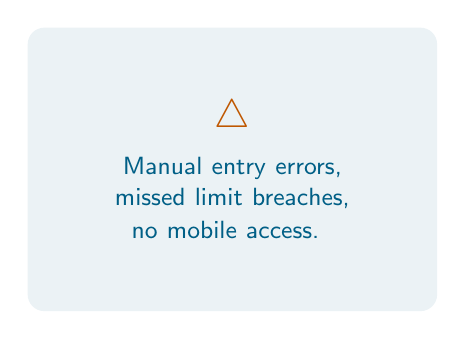
\begin{tikzpicture}
        \fill[utblue!8, rounded corners=6pt] (0,0) rectangle (5.2,3.6);
        \node[text width=4.8cm, align=center] at (2.6,1.8) {
          {\Large\color{utred} $\bigtriangleup$}\\[6pt]
          {\small\color{utblue}
            Manual entry errors,\\
            missed limit breaches,\\
            no mobile access.
          }
        };
      \end{tikzpicture}
  \end{columns}
\end{frame}

% ════════════════════════════════════════════════════════════════════════════════
%  4. OUR SOLUTION
% ════════════════════════════════════════════════════════════════════════════════
\setspeaker{[ALUMNO SLIDE 4]}
\begin{frame}{Our Solution}
  \accentrule
  \begin{columns}[T]
    \column{0.48\textwidth}
      \vspace{0.2cm}
      {\large\color{utblue} A lightweight, browser-based tool:}
      \vspace{0.4cm}
      \begin{itemize}\setlength\itemsep{9pt}
        \item \textbf{Visual dashboards} for historical KPIs
        \item \textbf{Automatic anomaly detection} by area
        \item \textbf{Telegram bot} for remote data entry
        \item \textbf{CSV-backed storage} --- no database needed
      \end{itemize}
      \vspace{0.4cm}
      {\small\color{utgray} Python $\cdot$ Streamlit $\cdot$ Telegram API}

    \column{0.48\textwidth}
      \includegraphics[width=\linewidth,height=5cm,keepaspectratio]%
        {Fotos/Screenshot From 2026-09-02 19-03-56.png}
      \piefig{Fig. 1 --- Dashboard overview: navigation panel and KPI chart.}
  \end{columns}
\end{frame}

% ════════════════════════════════════════════════════════════════════════════════
%  5. KPI TRACKING
% ════════════════════════════════════════════════════════════════════════════════
\setspeaker{[ALUMNO SLIDE 5]}
\begin{frame}{KPI Tracking}
  \accentrule
  \begin{columns}[T]
    \column{0.48\textwidth}
      \vspace{0.2cm}
      {\color{utblue}\textbf{Monthly historical analysis}}
      \vspace{0.3cm}
      \begin{itemize}\setlength\itemsep{8pt}
        \item Tracks consumption from \textbf{2021 to present}
        \item Automatic date parsing and sorting
        \item Single line chart --- \textbf{easy to read trend}
      \end{itemize}

    \column{0.48\textwidth}
      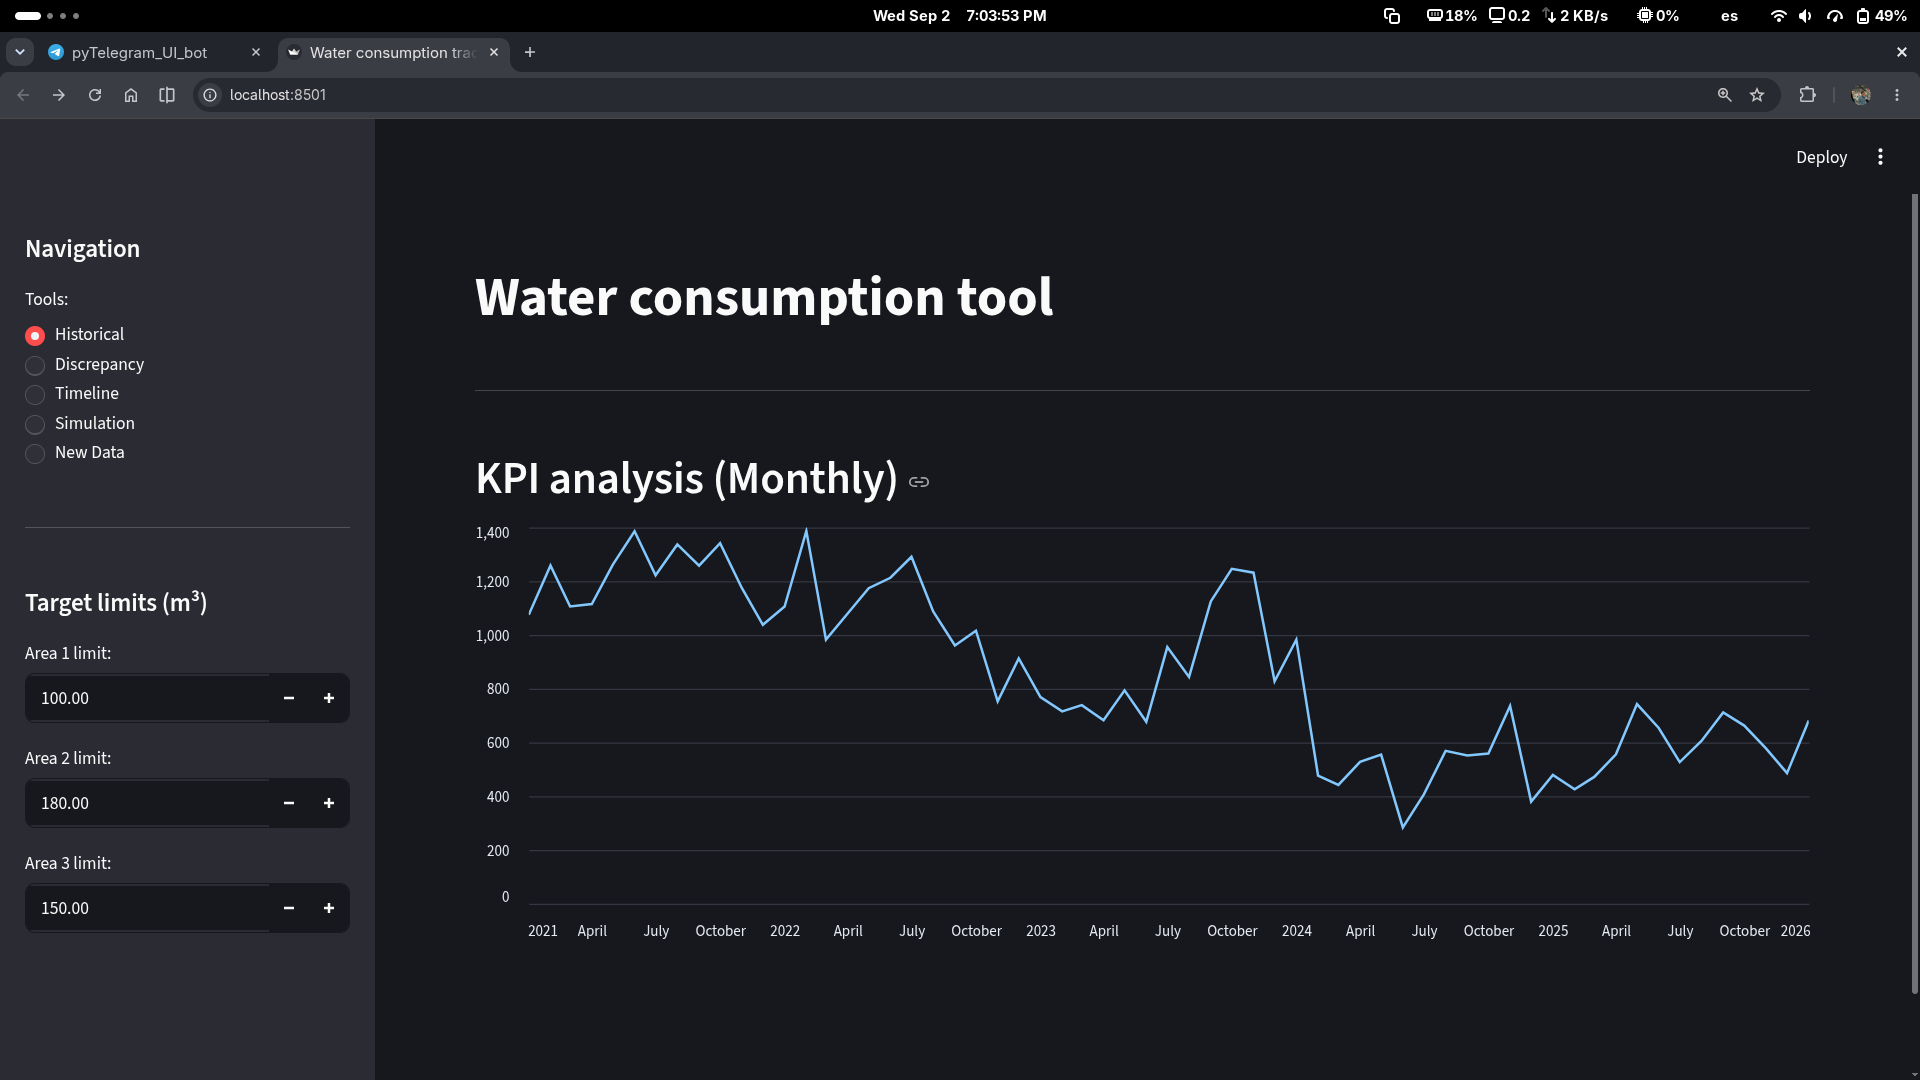
\includegraphics[width=\linewidth]{Fotos/Screenshot From 2026-09-02 19-03-56.png}
      \piefig{Fig. 2 --- Monthly KPI chart: total consumption 2021--2026.}
  \end{columns}
\end{frame}

% ════════════════════════════════════════════════════════════════════════════════
%  6. ANOMALY DETECTION
% ════════════════════════════════════════════════════════════════════════════════
\setspeaker{[ALUMNO SLIDE 6]}
\begin{frame}{Anomaly Detection}
  \accentrule
  \begin{columns}[T]
    \column{0.48\textwidth}
      \vspace{0.2cm}
      {\color{utblue}\textbf{Automatic limit breach detection}}
      \vspace{0.3cm}
      \begin{itemize}\setlength\itemsep{8pt}
        \item Configurable \textbf{per-area thresholds} (m\textsuperscript{3})
        \item Flags weeks with \textbf{negative Area 3} readings
        \item Anomalous weeks \textbf{highlighted in a table}
        \item Area 3 trend chart included for context
      \end{itemize}

    \column{0.48\textwidth}
      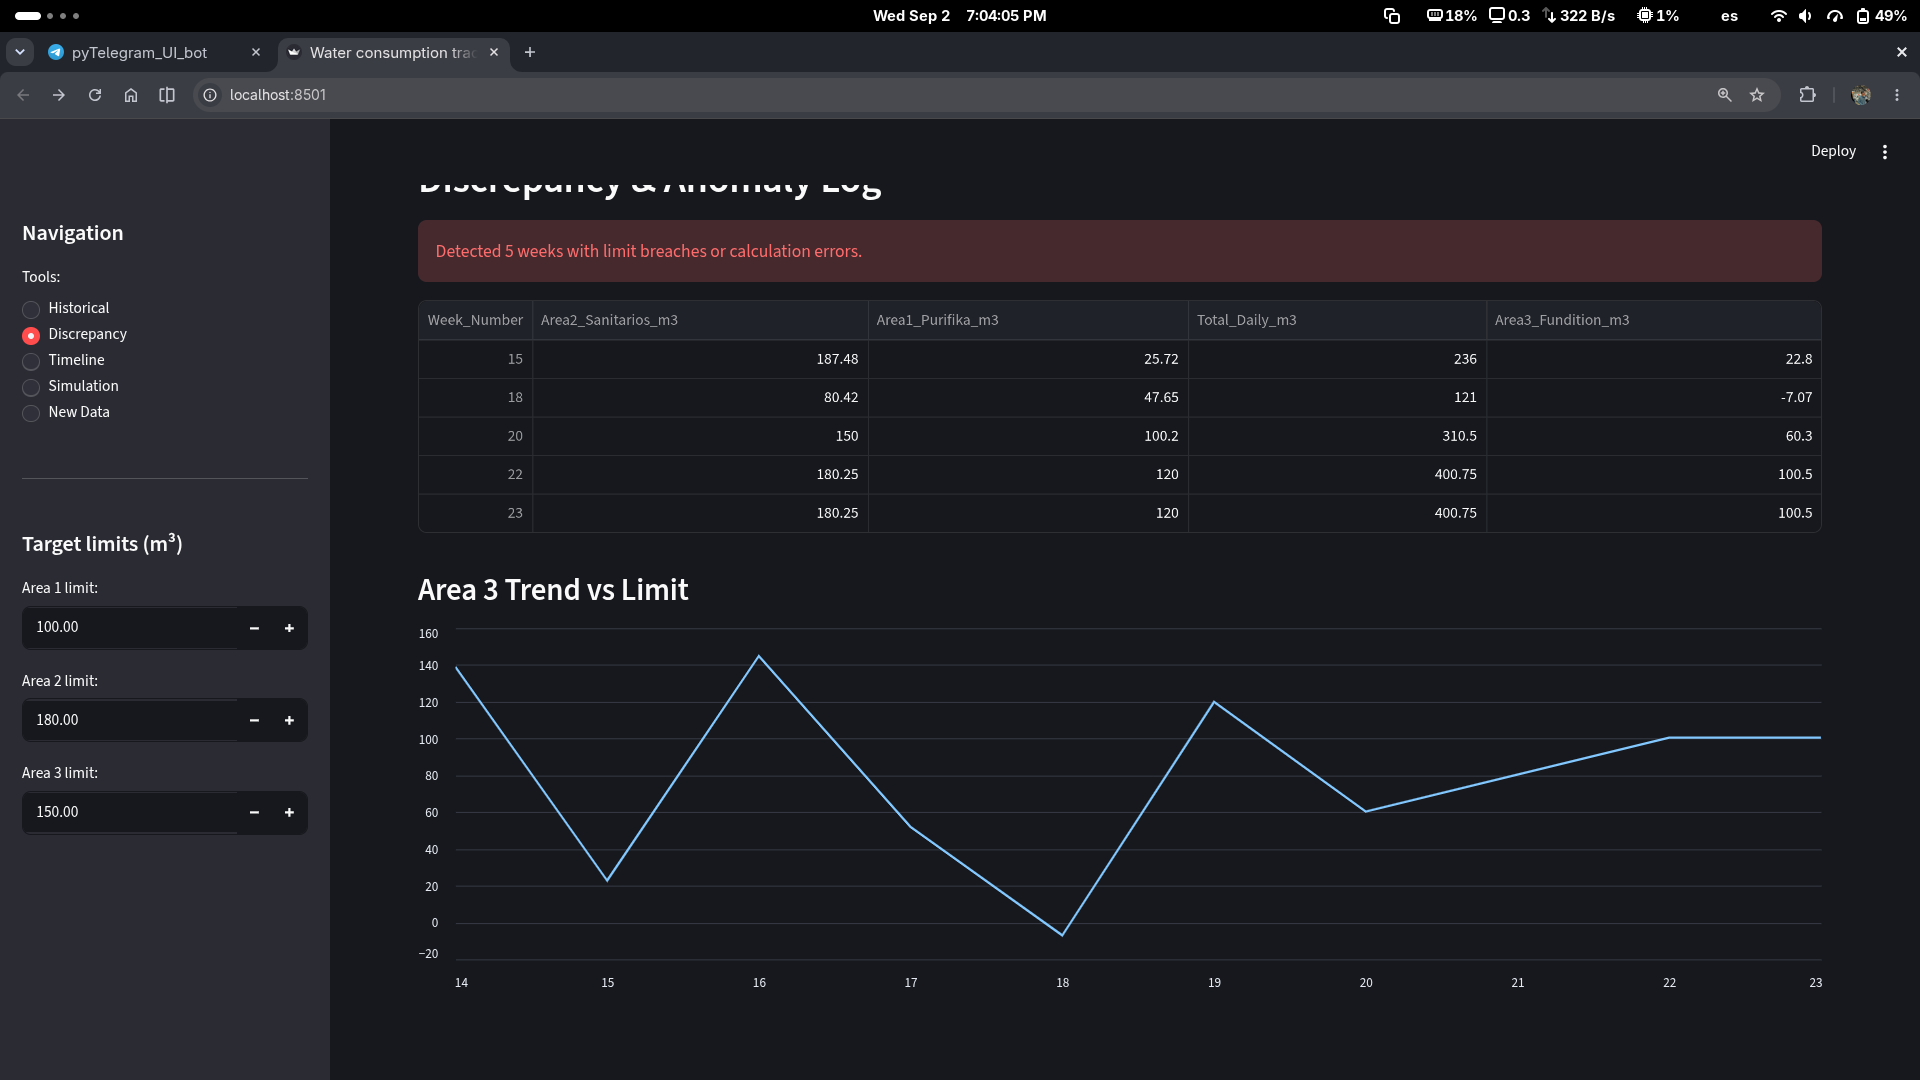
\includegraphics[width=\linewidth]{Fotos/Screenshot From 2026-09-02 19-04-07.png}
      \piefig{Fig. 3 --- Discrepancy log: flagged weeks and Area 3 trend.}
  \end{columns}
\end{frame}

% ════════════════════════════════════════════════════════════════════════════════
%  7. SHIFT TIMELINE
% ════════════════════════════════════════════════════════════════════════════════
\setspeaker{[ALUMNO SLIDE 7]}
\begin{frame}{Shift Timeline}
  \accentrule
  \begin{columns}[T]
    \column{0.46\textwidth}
      \vspace{0.3cm}
      {\color{utblue}\textbf{Day-by-day shift breakdown}}
      \vspace{0.4cm}
      \begin{itemize}\setlength\itemsep{8pt}
        \item Compares \textbf{Shift 1, 2 \& 3} simultaneously
        \item Interactive \textbf{timeframe slider} (days)
        \item \textbf{Pan} across any date window instantly
        \item Area chart reveals \textbf{peak consumption} patterns
      \end{itemize}

    \column{0.50\textwidth}
      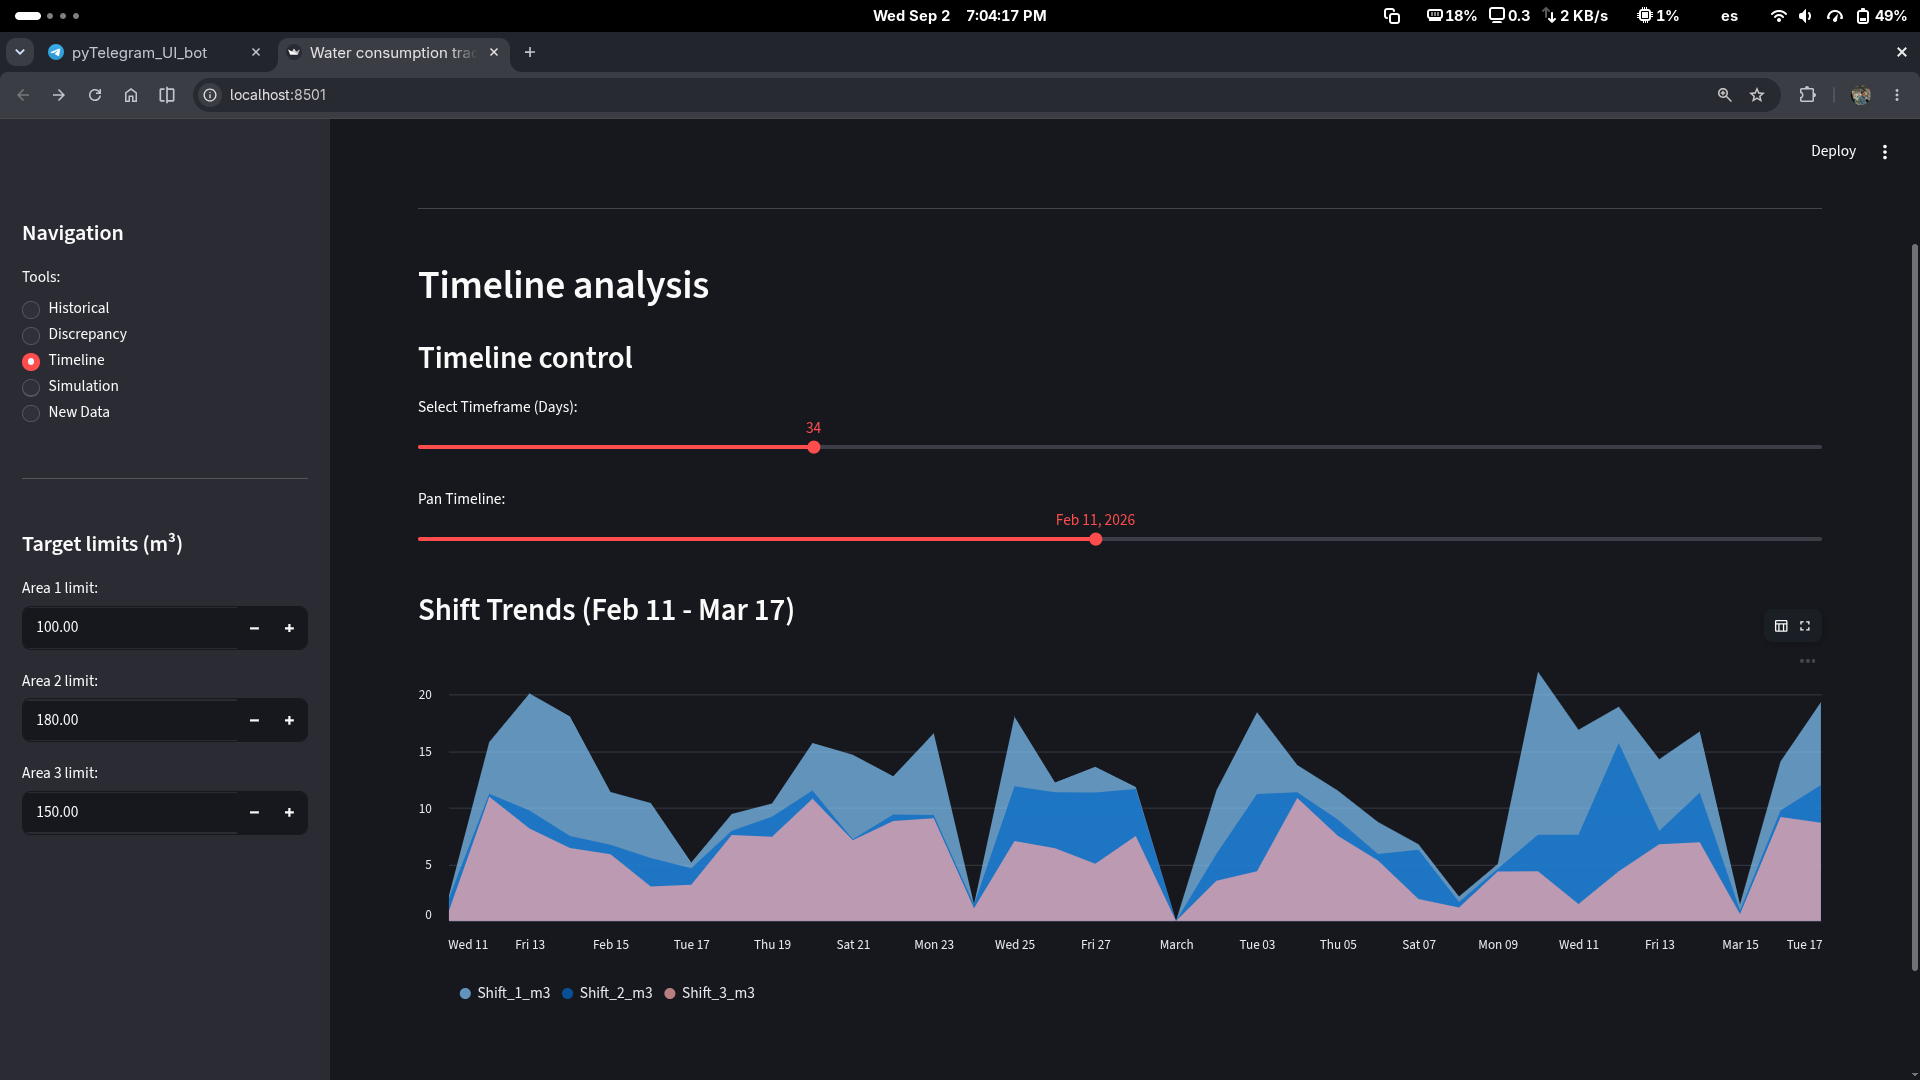
\includegraphics[width=\linewidth]{Fotos/Screenshot From 2026-09-02 19-04-18.png}
      \piefig{Fig. 4 --- Timeline: shift trends Feb 11 -- Mar 17, 2026.}
  \end{columns}
\end{frame}

% ════════════════════════════════════════════════════════════════════════════════
%  8. TELEGRAM
% ════════════════════════════════════════════════════════════════════════════════
\setspeaker{[ALUMNO SLIDE 8]}
\begin{frame}{Mobile Data Entry via Telegram}
  \accentrule
  \begin{columns}[T]
    \column{0.44\textwidth}
      \vspace{0.2cm}
      {\color{utblue}\textbf{No app installation needed}}
      \vspace{0.3cm}
      \begin{itemize}\setlength\itemsep{7pt}
        \item Send readings from \textbf{any phone}
        \item Two accepted formats:
        \vspace{3pt}
        \begin{itemize}
          \item {\scriptsize\texttt{21, 280, 80.5, 90.5}}
          \item {\scriptsize\texttt{semana 21 / total 280 / area1 80.5}}
        \end{itemize}
        \vspace{3pt}
        \item Dashboard \textbf{fetches on demand}
        \item Data previewed, then \textbf{saved with one click}
      \end{itemize}

    \column{0.52\textwidth}
      \includegraphics[width=\linewidth,height=5.4cm,keepaspectratio]%
        {Fotos/Screenshot From 2026-09-02 19-03-23.png}
      \piefig{Fig. 5 --- Telegram bot and import panel side by side.}
  \end{columns}
\end{frame}

% ════════════════════════════════════════════════════════════════════════════════
%  9. SIMULATION
% ════════════════════════════════════════════════════════════════════════════════
\setspeaker{[ALUMNO SLIDE 9]}
\begin{frame}{What-If Simulation}
  \accentrule
  \begin{columns}[T]
    \column{0.50\textwidth}
      \vspace{0.3cm}
      {\color{utblue}\textbf{Evaluate actions before implementing them}}
      \vspace{0.4cm}
      \begin{itemize}\setlength\itemsep{9pt}
        \item Describe a proposed conservation action
        \item Input estimated \textbf{weekly savings} (m\textsuperscript{3})
        \item Tool calculates \textbf{projected annual impact}
        \item Supports data-driven decisions with \textbf{no modeling required}
      \end{itemize}

    \column{0.46\textwidth}
      \vspace{0.2cm}
      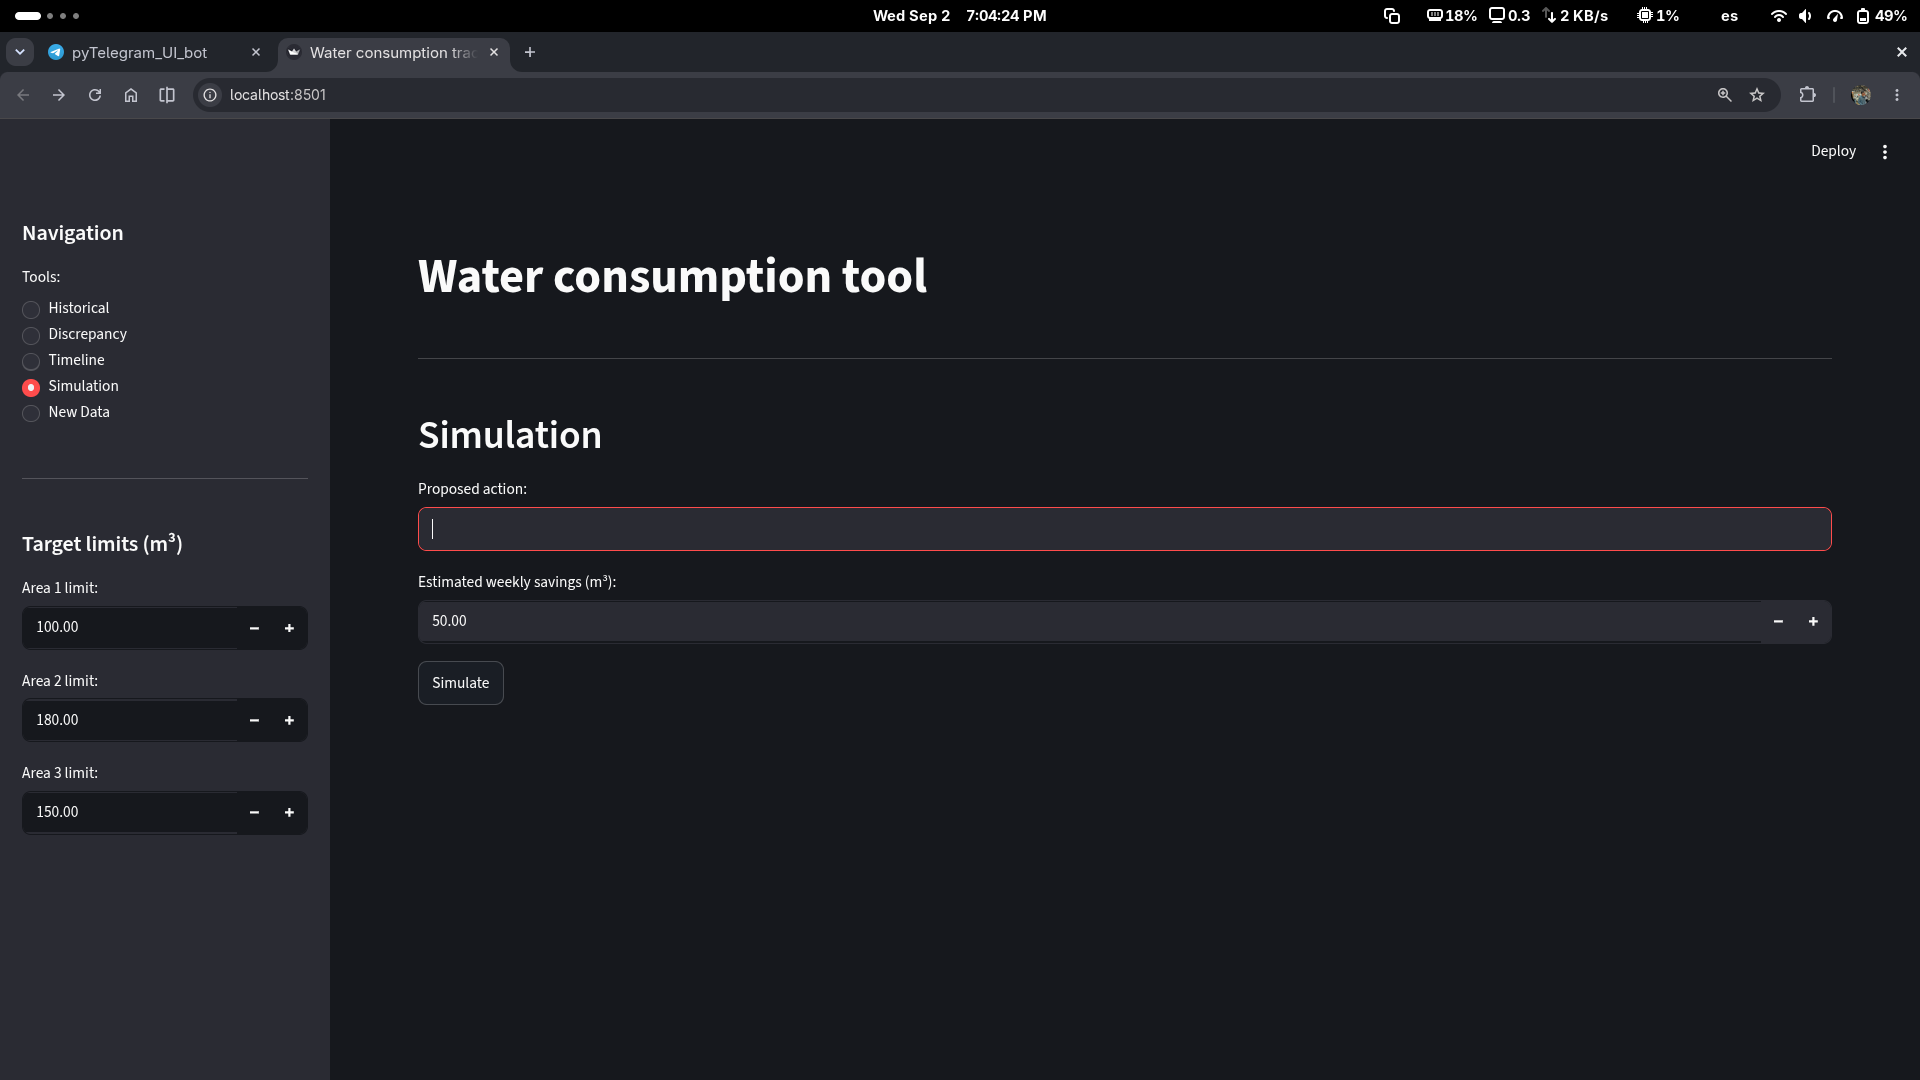
\includegraphics[width=\linewidth]{Fotos/Screenshot From 2026-09-02 19-04-25.png}
      \piefig{Fig. 6 --- Simulation panel: action input and annual KPI projection.}
  \end{columns}
\end{frame}

% ════════════════════════════════════════════════════════════════════════════════
%  10. SUMMARY
% ════════════════════════════════════════════════════════════════════════════════
\setspeaker{[ALUMNO SLIDE 10]}
\begin{frame}{Summary}
  \accentrule
  \vspace{0.2cm}
  \begin{columns}[T]
    \column{0.55\textwidth}
      \begin{tabular}{p{0.40\textwidth} p{0.48\textwidth}}
        \toprule
        \textbf{\color{utblue}Feature} & \textbf{\color{utblue}Capability} \\
        \midrule
        Historical KPIs   & Monthly trends since 2021      \\[3pt]
        Anomaly detection & 3 configurable area limits     \\[3pt]
        Shift timeline    & Day-level granularity          \\[3pt]
        Remote entry      & Telegram bot                   \\[3pt]
        Simulation        & Annual impact forecast         \\[3pt]
        Storage           & CSV --- portable, no setup     \\
        \bottomrule
      \end{tabular}

    \column{0.40\textwidth}
      \vspace{0.2cm}
      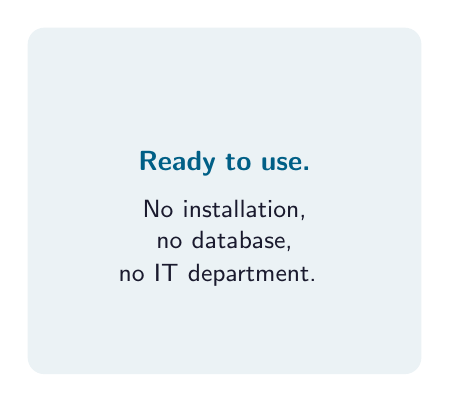
\begin{tikzpicture}
        \fill[utblue!8, rounded corners=6pt] (0,0) rectangle (5.0,4.4);
        \node[text width=4.6cm, align=center] at (2.5,2.2) {
          {\Large\color{utred} $\checkmark$}\\[8pt]
          {\color{utblue}\textbf{Ready to use.}}\\[6pt]
          {\small\color{textdark}
            No installation,\\
            no database,\\
            no IT department.
          }
        };
      \end{tikzpicture}
  \end{columns}
\end{frame}

% ════════════════════════════════════════════════════════════════════════════════
%  11. CLOSING
% ════════════════════════════════════════════════════════════════════════════════
\hidefooter
\begin{frame}[plain]
  \begin{tikzpicture}[remember picture, overlay]
    \fill[utblue] (current page.south west) rectangle ++(\paperwidth,{0.22\paperheight});
    \fill[utred]  (current page.south west) rectangle ++(\paperwidth,{0.04\paperheight});
  \end{tikzpicture}

  \vspace{1.2cm}
  \begin{center}
    {\Huge\bfseries\color{utblue} Thank You}

    \vspace{0.5cm}
    
\begin{tikzpicture}
      \draw[utred, line width=2pt] (0,0) -- (1.5,0);
      \draw[utlightblue, line width=2pt] (1.55,0) -- (2.4,0);
    \end{tikzpicture}

    \vspace{0.4cm}
    {\color{utgray}\small Questions?}

    \vspace{2.0cm}
    {\scriptsize\color{bgwhite}
      [ALUMNO 1] \quad$\cdot$\quad [ALUMNO 2] \quad$\cdot$\quad [ALUMNO 3]
    }
    {\scriptsize\color{bgwhite}
      \quad\textbar\quad [MATERIA] \quad\textbar\quad UT Austin
    }
  \end{center}
\end{frame}

\end{document}
